\chapter{The Transcorrelated Method for Multireference Problems}
\label{chap:binding}

This chapter is based in large part on the following upcoming publication:\\
\fullcite{haupt_sizeconsistent}

Images have been reused from this paper (with permission).

\section{Introduction}

In this chapter, we apply the new framework for the transcorrated method described in chapter \ref{chap:opt} to problems of multireference character and find these methods may yield non-physical results. We propose an updated workflow wherein we use conventional post-Hartree-Fock methods as input to Jastrow optimisation for TC-FCIQMC. Results suggest size-consistent results and rapid basis set convergence compared to conventional methods, with the binding curve of N$_2$ at \avtz being within chemical accuracy of experiment.

\section{Motivation}

A popular ``stress test'' for quantum chemistry methods is the binding curve of N$_2$. Highly accurate experimental results\supercite{leroyAccurate2006} exist to recreate the curve, allowing for a useful benchmark. At equilibrium, this system is essentially single reference in character, but as the bond is stretched, the system becomes strongly multireference, making it particularly challenging for many methods. As an example, we might consider standard \gls{CCSD}, which is a single-reference method, compared to FCIQMC which (within stochastic error) is exact. Figure \ref{fig:ccsd-vs-fciqmc-n2} shows the binding curve of N$_2$ with CCSD compared to FCIQMC, using \avtz. We see that CCSD is not stable at large bond lengths.

\begin{figure}[htbp]
    \centering
    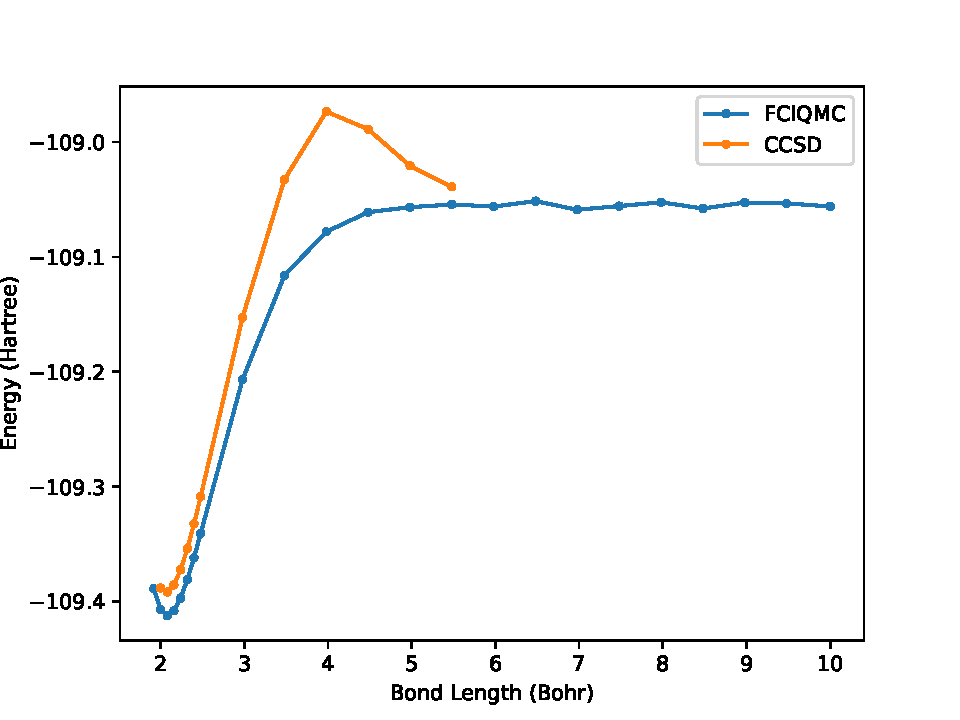
\includegraphics[width=0.8\textwidth]{figures/binding/N2_avtz_nontc}
    \caption{The binding curve for N$_2$ with the \avdz basis set. CCSD starts to decrease near 4 Bohr, which is nonphysical, whereas FCIQMC provides a more accurate curve. FCIQMC was done with 30 million walkers and HF-projected energy. The nonsmooth points in the dissociated region is due to stochastic error, and could be resolved with more walkers and a better trial wave function. CCSD did not converge at bond lengths larger than those shown.}
    \label{fig:ccsd-vs-fciqmc-n2}
\end{figure}

To see how well TC fares against such problems, consider the methodology outlined in chapter \ref{chap:opt}. We again use the same Jastrow factor as in equation \ref{eq:jastrow},
\begin{equation}
    \label{eq:jastrow-again}
    J = \sum_{i<j}^Nv(r_{ij}) + \sum_i^N\sum_I^{N_A}\chi(r_{iI}) + \sum_{i<j}^N\sum_I^{N_A}f(r_{ij}, r_{iI}, r_{jI}),
\end{equation}
with
\begin{equation}
    \label{eq:dtn-jastrow-ee-2}
    v(r_{ij})    = t(r_{ij},L_v)
                    \sum_{k} a_k r_{ij}^k ,
\end{equation}
\begin{equation}
    \label{eq:dtn-jastrow-en-2}
    \chi(r_{iI}) = t(r_{iI},L_\chi)
    \sum_{k} b_k r_{iI}^k ,
\end{equation}
\begin{equation}
    \label{eq:dtn-jastrow-een-2}
    f(r_{ij}, r_{i}, r_{j}) = t(r_{iI},L_f) t(r_{jI},L_f)
    \sum_{k,l,m} c_{klm}
    r_{ij}^k r_{iI}^l r_{jI}^m ,
\end{equation}
and the same cutoff functions $t(r,L) = (1-r/L)^3
\Theta(r-L)$. We also use the same objective function,
\begin{equation}
    \label{eq:varref-hf}
    \sigma_\mathrm{ref}^2 = \sum_{I\neq \mathrm{HF}}\bra{D_I}\htc\ket{D_\mathrm{HF}},
\end{equation}
Using this workflow with the xTC approximation, we calculate points along the binding curve of N$_2$, and find a non-physical ``dip'', as shown in figure \ref{fig:binding-dip}, similar to what CCSD exhibits in figure \ref{fig:ccsd-vs-fciqmc-n2}, albeit much more subtle.

\begin{figure}[htbp]
    \centering
    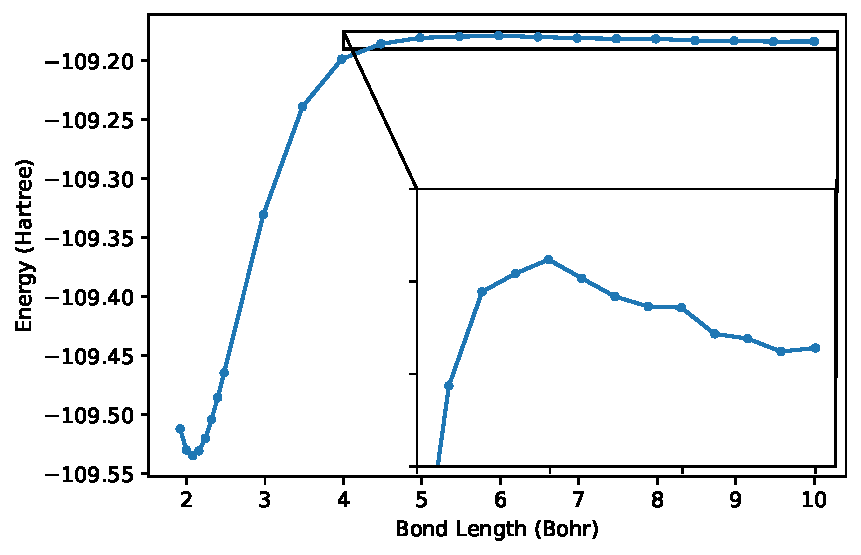
\includegraphics[width=0.8\textwidth]{figures/binding/inset_nontcfciqmc}
    \caption{The xTC-FCIQMC binding curve for N$_2$ with the \avtz basis set. While much smaller than that in figure \ref{fig:ccsd-vs-fciqmc-n2}, a non-physical dip is still present. This is apparent when zooming in on the curve, as shown in the inset.}
    \label{fig:binding-dip}
\end{figure}

This result has been verified for a few points with full TC (that is, with no approximations), which rules out xTC as the issue. Since the post-Hartree-Fock treatment was essentially at the FCI level, this implies that there is something wrong with the calculation of the Jastrow factors themselves. That is, our Hamiltonian is already ``corrupted'' before we even start the post-HF calculation.


\section{Resolving the Problem}

Based on the discussion in the previous section, it is likely that the transcorrelated workflow suffers from a single-reference bias. Indeed, the clear culprit is the Slater-Jastrow ansatz
\begin{equation}
    \label{eq:slater-jastrow}
    \Psi_\mathrm{SJ} = \e^J\Phi_\mathrm{HF},
\end{equation}
which affects the Jastrow optimisation and in turn the TC Hamiltonian $\htc = e^{-J}\hat H\e^J$.

We modify equation \ref{eq:slater-jastrow} to optimise for a multireference expansion,
\begin{equation}
    \label{eq:general-slater-jastrow}
    \Psi = \e^J\Phi_0
\end{equation}
where $\ket{\Phi_0}=\sum_I\ket{D_I}$. In practice, this modification results in two key changes in the workflow:
\begin{itemize}
    \item The objective function used during the VMC optimisation, equation \ref{eq:varref-hf}, needs to reflect the multireference ansatz. In particular, it will need to be changed to
    \begin{equation}
        \label{eq:varref-md}
        \sigma_\mathrm{ref}^2 = \sum_{I}\bra{D_I}\htc\ket{\Phi_0} - \bra{\Phi_0}\htc\ket{\Phi_0},
    \end{equation}
    which is evaluated in VMC by sampling
    \begin{equation}
        S_\mathrm{ref}^2 =
          \frac 1 {n_\mathrm{opt}-1}
          \sum_{n=1}^{n_\mathrm{opt}}
            \left| \frac {\hat H({\bm R}_n) \Psi({\bm R}_n)}
                         {\Psi({\bm R}_n)} - {\bar E}_\mathrm{ref}
            \right|^2.
    \end{equation}
    \item The density matrices used for xTC during integration must reflect this change as well. In particular, $\gamma_{p\dots}^{q\dots}=\bra{\Phi_0} a_{p\dots}^{q\dots}\ket{\Phi_0}$ in the equations in section \ref{sec:xtc}.
\end{itemize}

\subsection{Size Consistency}

One possible concern when studying problems like dissociation is that the method be size consistent. It is worth noting that one of the earliest Jastrow factors used for TC\supercite{boysCalculation1969} as well as in more recent work\supercite{cohenSimilarity2019} is given by
\begin{equation}
\label{eq:boyshandyjastrow}
J = \sum_{i<j} u(\bm r_i, \bm r_j)
\end{equation}
where
\begin{equation}
u(\bm r_i, \bm r_j) = \sum_{l,m,n}^{m+n+o\leq 6} c_{lmn}(\bar r_{iM}^m\bar r_{jN}^n+\bar r_{jM}^m\bar r_{iN}^n)\bar r_{ij}^l
\end{equation}
and $\bar r = r/(1+r)$.
However, notice that for $l=0$ and $n,m>0$, we can have non-vanishing gradients of $u$ for arbitrary distances between $N$ and $M$, and hence for systems $A$ and $B$ arbitrarily far apart we do not necessarily have
\begin{equation}
\label{eq:size-consistency}
e^{J_{A+B}}\ket{\Phi_{A+B}} = e^{J_0}(e^{J_{A}}\ket{\Phi_{A}})(e^{J_{B}}\ket{\Phi_{B}}),
\end{equation}
as $J_A$ will still act on system $B$, and vice versa. Here, $J_0$ is the electron-electron part of the Jastrow factor, $J_A$ the part involving nuclei in system $A$, and $J_B$ terms involving nuclei in system $B$.

In contrast to these previous works, our Jastrow ansatz, equation \ref{eq:jastrow-again}, first presented by Drummond, Towler and Needs,\supercite{drummondJastrow2004} vanishes when systems $A$ and $B$ are far apart due to the presence of the cutoff functions. Therefore, our Jastrow factor form does not suffer from this problem.

We must also ensure size consistency in our optimisation procedure. Assuming $\Phi_0$ is itself size consistent, it follows that for the given $J$, for non-interacting systems $A$ and $B$, the objective function, equation \ref{eq:varref-md}, $\sigma_\mathrm{ref}^2(A+B) = \sigma_\mathrm{ref}^2(A) + \sigma_\mathrm{ref}^2(B)$, where $\sigma_\mathrm{ref}^2(A)$ is the objective function for system $A$, and similarly for $B$. Hence, the parameters of the Jastrow factor should converge to the same values when treated as a non-interacting composite system as they would when treated as individual systems. Hence, our updated workflow is size consistent.

\subsection{Choices for Multireference Ansatzes}

We are now faced with the question of which choice of $\Phi_0$ is best. We present here three choices, and discuss their relative merits:
\begin{itemize}
    \item Using a FCIQMC wavefunction ansatz for $\Phi_0$. This is the most accurate one might get to the true solution, being essentially exact, but it is also computationally prohibitive for large systems. However, it is the most ``fool-proof'' proof-of-concept choice, can be treated as a blackbox (no need to choose an active space), and we might simply end the calculation early to get the most important components of the CI vector. In this chapter, we use a ``snapshot'' of the wave function at the end of a non-TC-FCIQMC calculation, and use the associated 1RDM calculated by the ``replica trick'' presented in section \ref{sec:fciqmc_rdm}. Since our TC calculation is xTC-FCIQMC, using FCIQMC as the ansatz for $\Phi_0$ might be dubbed ``circular'' and actually does not worsen the computational scaling of the methodology. Of course, if we choose to use e.g. xTC-DCSD as our TC method, then the computational bottleneck is non-TC-FCIQMC, before we even begin transcorrelation. We will refer to Jastrow factors optimised with this ansatz as ``FCIQMC-Jastrows''.
    \item Using a CASSCF wavefunction ansatz for $\Phi_0$. In this method, the orbitals are also modified. It is a compromise compared to the FCIQMC approach, though still quite costly, is not a blackbox method, and a greater percentage of the wavefunction might be stored in the CI vector (since only a smaller subset of the orbitals are considered). We will refer to Jastrow factors optimised with this ansatz as ``CASSCF-Jastrows''.
    \item Using a CASCI wavefunction ansatz for $\Phi_0$. Of the methods presented here, this is the least costly while still potentially capturing much of the static correlation needed and being relatively blackbox.\supercite{levineCAS2021} This is probably the most realistic choice for large-scale problems. We will refer to Jastrow factors optimised with this ansatz as ``CASCI-Jastrows''.
\end{itemize}
We refer to the Jastrow factors optimised with the restricted HF ansatz described in the previous section as ``RHF-Jastrows''.\footnote{Unrestricted HF along with spin-dependent Jastrow factors are the subject of a future work.}

\section{Trial Wavefunctions in TC-FCIQMC}
\begingroup
\def\trial {\Phi_\mathrm{trial}}
\def\evec {\Phi_\mathrm{FCIQMC}}
Another challenge when studying multireference problems with FCIQMC is noise in the projected energy. Here we generalise the discussion on trial wavefunctions presented in section \ref{sec:fciqmc_energy_estimators}.

Consider a TC-FCIQMC calculation, where we wish to solve for the eigenvalue of the ground state $\Phi$ for the TC Hamiltonian $\htc$. Conventionally, the projected energy can be written
\begin{equation}
    E_\mathrm{proj} = \frac{\bra\trial\htc\ket\evec}{\braket{\trial}{\evec}}
\end{equation}
where $\ket\evec$ is the estimate of the wave function according to the FCIQMC algorithm, and $\ket\trial$ is the trial wave function. If we write $\ket\evec$ as a sum of the exact wave function $\ket{\Phi}$ plus some error $\ket\delta$, we have
\begin{align}
    E_\mathrm{proj} &= \frac{\bra\trial\htc\ket{\Phi+\delta}}{\braket{\trial}{\Phi+\delta}} \\
    &= \frac{E_0\braket{\trial}{\Phi}+\bra\trial\htc\ket{\delta}}{\braket{\trial}{\Phi}+\braket{\trial}{\delta}}
\end{align}
where $E_0$ is the exact ground-state energy.
If $\ket\trial$ is the left eigenvector, then $\bra\trial\htc\ket{\delta}=(\htc^\dag\ket\trial)^\dag\ket{\delta}=E_0\braket{\trial}{\delta}$, so
\begin{align}
    E_\mathrm{proj} &= \frac{E_0\braket{\trial}{\Phi}+E_0\braket{\trial}{\delta}}{\braket{\trial}{\Phi}+\braket{\trial}{\delta}}\\&=E_0\frac{\braket{\trial}{\Phi}+\braket{\trial}{\delta}}{\braket{\trial}{\Phi}+\braket{\trial}{\delta}}\\&=E_0,
\end{align}
i.e. if our trial wavefunction is the left eigenvector of $\htc$, then $E_\mathrm{proj}=E_0$.

In standard FCIQMC, we take the top $N_T$ determinants at some point of a calculation, form a subspace by constructing a $N_T\times N_T$ trial space $H_\mathrm{trial}$, diagonalise it exactly, and use the eigenvector as an approximation to the exact one, to be used as $\ket\trial$ in the calculation of the projected energy. As $H$ is Hermitian, taking the left or the right eigenvector is irrelevant. To get the left eigenvector in an equivalent way would involve doing a FCIQMC calculation on $\htc^\dag$, but this is costly and instead we find taking the left eigenvector of the subspace from $\htc$ to be a good approximation, as the two typically have similar top determinants. Moreover, this method gives the correct energy as long as the trial wavefunction has nonzero overlap with the true eigenvector, so even if our choice is not perfect, it will still give the correct answer, and likely with a smaller error compared to using the Hartree-Fock determinant.

\endgroup

As an example of the effectiveness of this approach, consider a highly dissociated point in the binding curve of the nitrogen molecule. This is shown in figure \ref{fig:trial_projected_energy}, specifically at $10$ Bohr with the \avtz basis set and $10^8$ walkers. For this calculation, FCIQMC-Jastrows were used.
\begin{figure}[htbp]
    \centering
    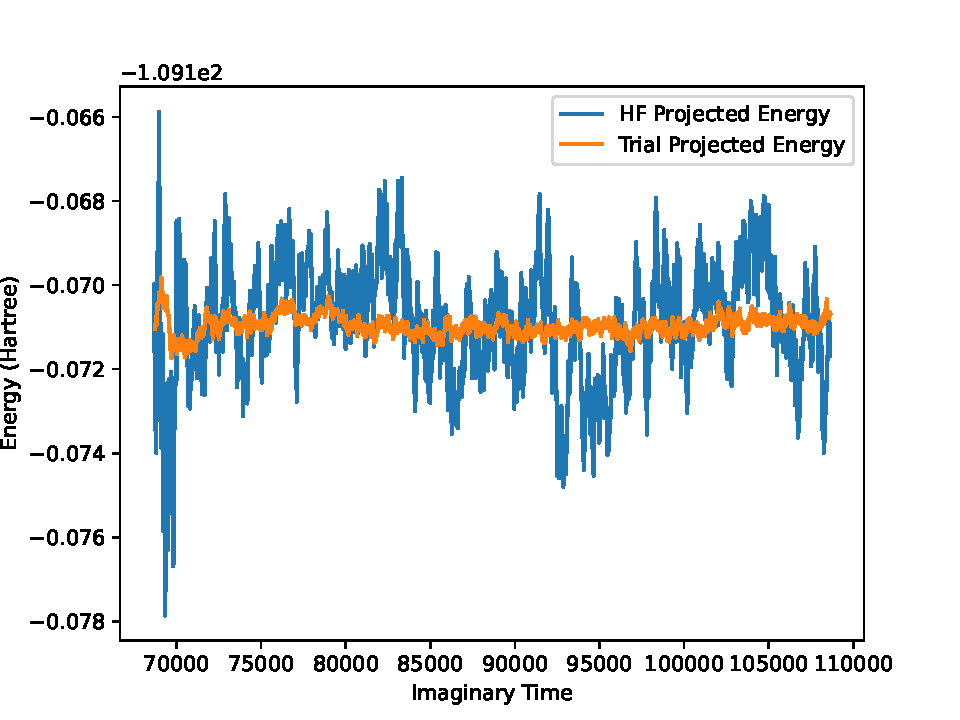
\includegraphics[width=0.8\textwidth]{figures/binding/trial_v_projE.pdf}
    \caption{The HF-projected and trial-projected energy trajectories in imaginary time for N$_2$ with a separation of $10$ Bohr with the \avtz basis set and the Jastrow factor optimised for the variance of the FCIQMC energy. The calculation was done with $10^8$ FCIQMC walkers. This is a highly dissociated and hence multireference state. The trial-projected energy uses the top 10 determinants but substantially improves the rate of convergence when compared to the HF projected energy.}
    \label{fig:trial_projected_energy}
\end{figure}
We can see from this figure that using the trial-projected energy even with just a few determinants allows us to much more easily handle highly multireference problems. Thus, trial wave functions are used throughout the rest of this chapter.

\section{Results}
\subsection{Computational Details}

We calculate the energy of the nitrogen molecule across multiple bond lengths, ranging from $1.92$ to $10$ Bohr. We use the \avtz basis set, which contains diffuse functions for long-range correlations while still being a modest size. We calculate the non-TC CI vectors and \glspl{1RDM} for each geometry with FCIQMC (using \neci),\supercite{gutherNECI2020} CASSCF (using \molpro),\supercite{wernerMOLPRO,wernerMolpro2012,wernerMolproQuantumChemistry2020} and CASCI (using \pyscf).\supercite{sunPySCF2018} The CI vector is then used in the objective function for optimising the Jastrow factor with VMC using \casino.\supercite{needsVariational2020} Using the optimised Jastrow factor and 1RDM, we then calculate the relevant integrals for the xTC Hamiltonian using \pytchint. Finally, xTC-FCIQMC is performed on these integrals with \neci. Each geometry is calculated independently; that is, the Jastrow factor is optimised for each geometry separately. In order to keep memory usage manageable, we cutoff the number of determinants in our CI vector to be $100$. Even at the dissociated limit, the number of relatively-highly-weighted determinants is around $20$, so $100$ should be enough to capture the static correlation for the VMC optimisation.

Next, we also calculate the vertical excited-state energies using this workflow for a few states of the nitrogen and ammonia (NH$_3$) molecules with CASSCF- and CASCI-Jastrows. Excited states are also challenging multireference problems. Moreover, we optimise the Jastrow factors in a state-specific manner. That is, for some excited state $\Phi_\mathrm{ex}$, our ansatz becomes $\Psi_\mathrm{ex} = \e^J\Phi_\mathrm{ex}$, thereby modifying our workflow slightly to optimise specifically for that state, as well as using its 1RDM for the xTC approximation. Naturally, the xTC-FCIQMC calculation will be targeting this state. For cases where a triplet excited state of the same symmetry is lower in energy than a singlet excited state, the FCIQMC calculation will collapse to the triplet state. To overcome this, we use a spin-penalty term to target the singlet excited state.\supercite{weserSpin2022}

For the N$_2$ binding curve, we compare against the highly accurate experimental curve determined in reference \citenum{leroyAccurate2006}, and as a benchmark we compare against F12 calculations, performed in \molpro.\supercite{wernerMOLPRO,wernerMolpro2012,wernerMolproQuantumChemistry2020} For excited states we compare against extrapolated FCI calculations reported in reference \citenum{loosMountaineering2018}.

\subsection{Binding Curves}

As illustrated in figure \ref{fig:binding-curves-full-diss}, we obtain a qualitatively-correct binding curve for the nitrogen molecule using any of the Jastrow factors, besides the RHF-Jastrow. Shown in that figure is also a zoom-in on the dissociated limit, indicating the RHF-Jastrow curve is the only one exhibiting the pathological ``dip'' behaviour. The remaining nonphysical behaviour amounts to noise, which has a few potential sources:
\begin{itemize}
    \item The optimisation of the Jastrow factor is done with VMC, a stochastic algorithm. As described in \autoref{chap:opt}, VMC optimisation for the TC method is complex, and as of yet has not been done on strongly multireference problems. Since the optimisation is done independently for each point along the binding curve, this may lead to some noise.
    \item The FCIQMC calculations are also stochastic, and this may also lead to some noise, particularly in the dissociated limit when not using a multideterminantal trial wave function.
    \item In the case of the FCIQMC-Jastrow, even the non-TC calculation prior to Jastrow optimisation is stochastic. In this case, the CI vector and 1RDM collected from the non-TC-FCIQMC calculation is done so at only a snapshot in imaginary time: right at the end of the calculation. One way to reduce this noise (not explored here) would be to average these values over imaginary time.
\end{itemize}
Thus, we can conclude that the biggest problem with the TC workflow has been resolved in three ways by introducing a multireference Jastrow optimisation (and 1RDM for the xTC approximation).

\begin{figure}[htbp]
    \centering
    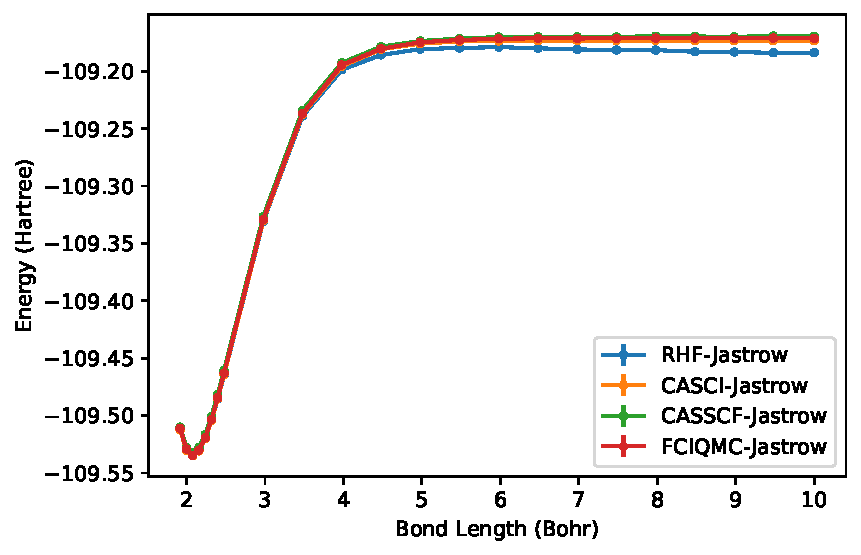
\includegraphics[width=0.8\textwidth]{figures/binding/all_binding_curves}
    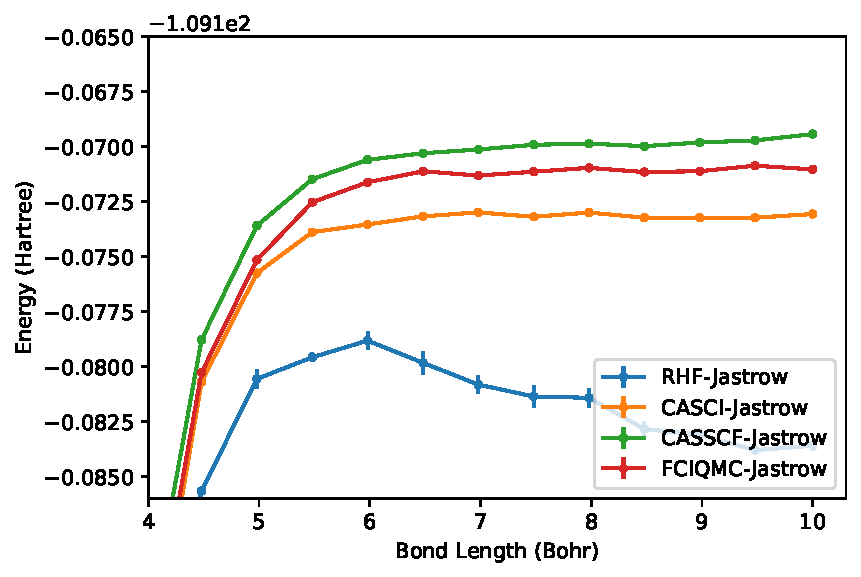
\includegraphics[width=0.8\textwidth]{figures/binding/all_binding_curves_dissociated}
    \caption{xTC-FCIQMC energies for the nitrogen dimer for various points along its binding curve, between 1.92 and 10 Bohr radii. Calculations were performed with the \avtz basis set. Four choices for Jastrow factors are presented. The forms for the actual Jastrow factor $J$ is the same, but the value for $\ket{\Phi}$ in the ansatz $\ket\Psi=\e^J\ket\Phi$ is different. The choices are: RHF-Jastrow (blue), CASCI-Jastrow (orange), CASSCF-Jastrow (green) and the FCIQMC-Jastrow (red). The top panel shows the full binding curve, while the bottom panel shows the dissociated limit. Notice that except for the RHF-Jastrow curve, these Jastrow factors result in qualitatively-correct xTC-FCIQMC binding curves.
    }
    \label{fig:binding-curves-full-diss}
\end{figure}

We now consider the binding curve at the equilibrium geometry (taken to be $2.08$ Bohr radii). Such a zoom-in is shown in figure \ref{fig:binding-curves-minimum}. Since N$_2$ is largely single-reference in this region, we expect all of the curves, including that with the RHF-Jastrow, to approximately be equal there. Relative to the RHF-Jastrow curve,
\begin{itemize}
    \item The CASCI-Jastrow curve uses the same orbitals and uses only a small subspace of the full CI space, and is indeed strongly single-reference in this region. As a result, this curve is almost identical to the RHF-Jastrow curve in the region around the minimum.
    \item The CASSCF-Jastrow curve has a noticeable shift of about $2.8$ mHa. While not expected, since the TC method is nonvariational we cannot guarantee a more complete wave function description to necessarily lead to a lower energy value. However, notice in the bottom panel of figure \ref{fig:binding-curves-full-diss} the CASSCF-Jastrow curve is shifted upwards relative to the CASCI-Jastrow curve by about the same amount, so in relative terms this is actually acceptable.
    \item The FCIQMC-Jastrow is slightly higher in energy compared to the RHF- and CASCI-Jastrow curves near the minimum, and similarly above the CASCI-Jastrow curve at dissociation. Since it shares the same orbitals as the CASCI-Jastrow curve, and we are primarily concerned with static correlation at this part of the workflow, we expect the FCIQMC-Jastrow curve to have a similar shape, and indeed it does. Possible sources of differences are: stochastic noise and having more flexibility to capture the full wave function (especially relevant at dissociation).
\end{itemize}

\begin{figure}[htbp]
    \centering
    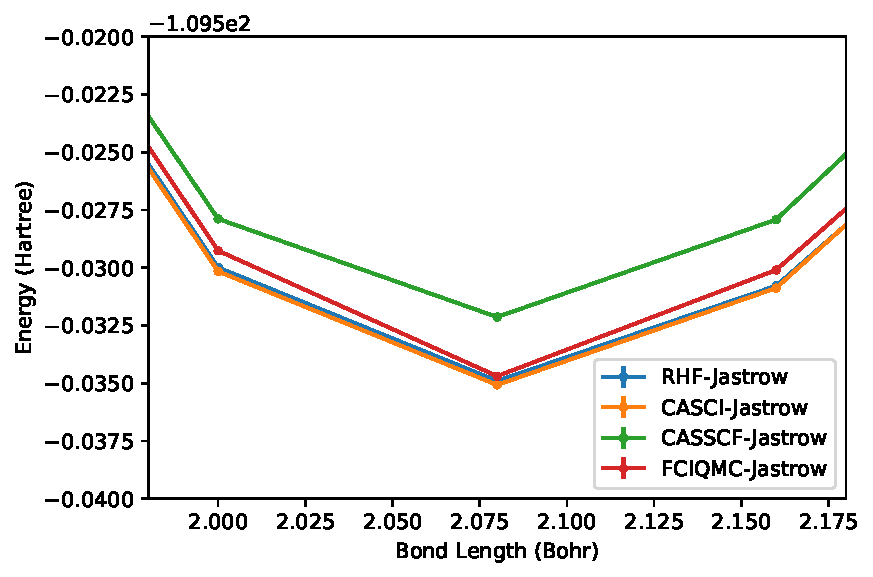
\includegraphics[width=0.8\textwidth]{figures/binding/all_binding_curves_min}
    \caption{The N$_2$ binding curves at \avtz for the RHF- (blue), CASCI- (orange), CASSCF- (green) and FCIQMC-Jastrow (red), zoomed in near equilibrium. Here, the problem is strongly single-reference and hence we expect all curves to be similar. However, the CASSCF-Jastrow curve is shifted upwards relative to the CASCI-Jastrow curve by about $2.8$ mHa, but this is compensated for at dissociation.}
    \label{fig:binding-curves-minimum}
\end{figure}

Naturally, we also wish to determine how accurate our calculations are. This is easy to verify for the extremes, as we can directly compare against HEAT.\supercite{fellerSurvey2008} However, we also want to evaluate the accuracy of the rest of the binding curve. For this, we test against an accurate fit to experimental spectroscopic data which includes high-energy dissociated data.\supercite{leroyAccurate2006} Since we are only interested in relative energies, we normalise all curves to be zero at $10$ Bohr radii, and subtract the experimental values. The result of this is shown in figure \ref{fig:binding-curves-experiment}.

\todo{discussion of results}

\begin{figure}[htbp]
    \centering
    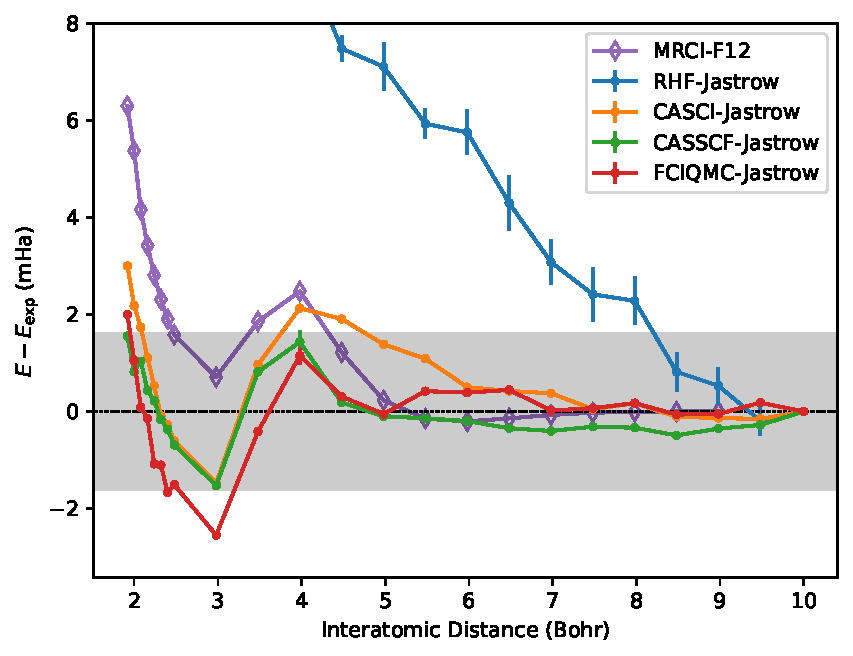
\includegraphics[width=0.8\textwidth]{figures/binding/residuals}
    \caption{Binding curves for each Jastrow factor optimisation strategy relative to the experimental fit from reference \citenum{leroyAccurate2006}. All curves are normalised such that the energy at $10$ Bohr radii is zero, except for MRCI-F12 where energy is set to zero at $8.98$ Bohr radii (past this, it did not converge). The shaded region represents $1.6$ mHa, so-called ``chemical accuracy''. We see that most of the curves for the multirefence Jastrow optimisations are within chemical accuracy, outperforming MRCI-F12. Note that while the relative values are below experiment for some regions (notably around $3$ Bohr), all absolute values are still above the HEAT result for N$_2$ (and thus can be considered variational).}
    \label{fig:binding-curves-experiment}
\end{figure}

We find that the CASCI- and FCIQMC-Jastrow curves are all within chemical accuracy (1.6 mHa) for most of the binding curve and the CASSCF-Jastrow entirely within chemical accuracy when compared against experiment, all of them outperforming MRCI-F12. It is worth noting, however, that unlike MRCI-F12, our multireference Jastrow factors are not uniformly above experiment.

% Another worthwhile check is how accurate the atomisation energy is, taking the extremely dissociated limit ($10$ Bohr radii) as twice the energy of the atom. This is shown in table \ref{tbl:binding-atomisation-energies}. \todo{discussion}

\todo{atomisation energies comparison against experiment and HEAT}


\begin{table}[!h]
    \centering
        \begin{tabular}{c|c}
            Jastrow Factor & Atomisation Energy (mHa) \\
            \hline
            CASCI & \todo{...} \\
            CASSCF & \todo{...} \\
            FCIQMC & \todo{...} \\
            \bottomrule
            HEAT\supercite{fellerSurvey2008} & \todo{...} \\
            Experiment\supercite{leroyAccurate2006} & \todo{...}
        \end{tabular}
    \caption{\todo{table of atomisation energies, mention also the HEAT result, mention RHF is meaningless because of dip}}
    \label{tbl:binding-atomisation-energies}
\end{table}


\todo{also include a table about just ``how size-consistent'' the results actually are.}

\begin{table}[!h]
    \centering
    \begin{tabular}{c|c}
        Jastrow Factor & $\sum E_\mathrm{atom} - E_\mathrm{molecule}(r=10)$ (mHa) \\
        \hline
        CASCI & \todo{...} \\
        CASSCF & \todo{...} \\
        FCIQMC & \todo{...}
    \end{tabular}
    \caption{\todo{error for size Consistency, again including RHF is meaningless because of the dip}}
    \label{tbl:size-consistency}
\end{table}


\subsection{Excitation Energies}
\todo{mention can target the exact state(s) in question}


\begin{table}[h!]
\centering
\begin{threeparttable}
\begin{tabular}{c|cccc|c}
\multicolumn{6}{c}{\textbf{Dinitrogen}} \\
State & Method & \avdz & \avtz & \avqz & Benchmarks \\
\hline
\multirow{3}{*}{$^1\Pi_g$}
& non-TC exFCI\tnote{a} & 345.8  &  & \todo{} & \todo{exp1}\tnote{b} \\
& CASCI-xTC    & 341.86(4) &  & \todo{} & \todo{exp2}\tnote{c}  \\
& CASSCF-xTC   & 340.729(3) &  & \todo{} & \todo{th1}\tnote{d}  \\
\hline
\multirow{3}{*}{$^1\Sigma_u^-$}
& non-TC exFCI\tnote{a}       & &    & \todo{}   & \multirow{3}{*}{\todo{}} \\
& CASCI-xTC          & &    & \todo{}   &  \\
& CASSCF-xTC         & &    & \todo{}   &  \\
\hline
\multirow{3}{*}{$^1\Delta_u$}
& non-TC exFCI\tnote{a}       & &    & \todo{}   & \multirow{3}{*}{\todo{}} \\
& CASCI-xTC          & &    & \todo{}   &  \\
& CASSCF-xTC         & &    & \todo{}   &  \\
\hline
\multirow{3}{*}{$^3\Sigma_u^+$}
& non-TC exFCI\tnote{a}       & &    & \todo{}   & \multirow{3}{*}{\todo{}} \\
& CASCI-xTC          & &    & \todo{}   &  \\
& CASSCF-xTC         & &    & \todo{}   &  \\
\hline
\multirow{3}{*}{$^3\Pi_g$}
& non-TC exFCI\tnote{a}       & &    & \todo{}   & \multirow{3}{*}{\todo{}} \\
& CASCI-xTC          & &    & \todo{}   &  \\
& CASSCF-xTC         & &    & \todo{}   &  \\
\hline
\multirow{3}{*}{$^3\Delta_u$}
& non-TC exFCI\tnote{a}       & &    & \todo{}   & \multirow{3}{*}{\todo{}} \\
& CASCI-xTC          & &    & \todo{}   &  \\
& CASSCF-xTC         & &    & \todo{}   &  \\
\bottomrule
\end{tabular}
\begin{tablenotes}
    \item[a] Taken from reference \citenum{loosMountaineering2018}.
    \item[b] Experimental value, reference \todo{...}.
    \item[c] Experimental value, reference \todo{...}.
    \item[d] Theoretical value, reference \todo{...}.
\end{tablenotes}
\end{threeparttable}
\caption{\todo{Comparison of methods and experimental values for different states.}}
\label{tbl:excitation-energies-n2}
\end{table}

\begin{table}[h!]
\centering
\begin{tabular}{c|cccc|c}
\multicolumn{6}{c}{\textbf{Ammonia}} \\
State & Method & \avdz & \avtz & \avqz & Experiment \\
\hline
\multirow{3}{*}{$^1\Pi_g$}
& non-TC exFCI     & &  & val 3 & \multirow{3}{*}{\todo{exp}} \\
& CASCI-xTC   & &  & val 1 &  \\
& CASSCF-xTC  & &  & val 2 &  \\
\hline
\multirow{3}{*}{$^3\Sigma_g$}
& \todo{}       & &    & \todo{}   & \multirow{3}{*}{\todo{}} \\
& \todo{}       & &    & \todo{}   &  \\
& \todo{}       & &    & \todo{}   &  \\
\end{tabular}
\caption{\todo{Comparison of methods and experimental values for different states.}}
\label{tbl:excitation-energies-nh3}
\end{table}

% \begin{table}[htbp]
%     \centering
%     \begin{tabular}{c|cccc}
%         % \multicolumn{5}{*}{Dinitrogen} \\
%         % \hline
%         \multicolumn{5}{c}{Dinitrogen} \\
%         \hline
%         \multirow{7}{*}{\rotatebox[origin=c]{90}{CASCI-xTC}} & State & \avdz & \avtz & \avqz \\
%         \hline
%         % \multirow{2}{*}{\rotatebox[origin=c]{90}{CASCI}} & State & \avdz & \avtz & \avqz \\
%         \cline{2-5}
%         & $^1\Pi_g$ & & & \\
%         & $^1\Sigma_u^-$ & & & \\
%         & $^1\Delta_u$ & & & \\
%         & $^3\Sigma_g^+$ & & & \\
%         & $^3\Pi_g$ & & & \\
%         & $^3\Delta_u$ & & & \\
%         % \hline
%         \hline
%         \multirow{7}{*}{\rotatebox[origin=c]{90}{CASSCF-xTC}}
%         & $^1\Pi_g$ & & & \\
%         & $^1\Sigma_u^-$ & & & \\
%         & $^1\Delta_u$ & & & \\
%         & $^3\Sigma_g^+$ & & & \\
%         & $^3\Pi_g$ & & & \\
%         & $^3\Delta_u$ & & & \\
%         &
%         $^1\Sigma_g^+$ & & & \\
%         % \cline{2-5}
%     \end{tabular}
%     \caption{\todo{excitation energies for N2, in mHa}}
%     \label{tbl:excitation-energies-n2}
% \end{table}

% \begin{table}[htbp]
%     \centering
%     NH$_3$, CASCI-Jastrow \\
%     \begin{tabular}{c|c|c|c}
%         State & \avdz & \avtz & \avqz \\
%         \hline
%          & & & \\
%     \end{tabular} \\
%     NH$_3$, CASSCF-Jastrow \\
%     \begin{tabular}{c|c|c|c}
%         State & \avdz & \avtz & \avqz \\
%         \hline
%          & & & \\
%     \end{tabular}
%     \caption{\todo{excitation energies for NH3, in mHa}}
%     \label{tbl:excitation-energies-nh3}
% \end{table}

\section{Conclusion and Outlook}
\todo{make sure to mention the cutoff analysis and constructing Jastrow factors from atomic Jastrow factors. Mention ECPs, since it's already been submitted...}
\todo{TC-CAS...}
\todo{self-consistent TC (i.e. feed back into itself)}
